\section{Skeleton pruning and holes closing (Optional)}

\subsection{Introduction}
Depending on the roughness and thickness of the tubes in the raw data the computed skeleton may contain false positive short branches and/or false positive small loops. These can eventually be removed by a process called "pruning". We will test the different pruning algorithms implemented in \ijmenu{Plugins > Skeleton > Analyze Skeleton (2D/3D)}.

\subsection{Workflow}

\begin{description}
\item[End-point pruning]\hfill\\
Remove all branches containing exactly one end-point by checking the "Prune ends" option in \ijmenu{Plugins > Skeleton > Analyze Skeleton (2D/3D)}. Carefully examine the image and check whether the pruning is always working as you would expect (see also figure ~\ref{fig:prune}).
\begin{figure}[h!]
  \caption{Skeleton annotation and pruning. Slab voxels are white, junction voxels are red and end-point voxels are blue. Images are projections of 3D data and were subject to different processing steps: (Left) Skeletonization => Analysis. (Center Left) Skeletonization => Analysis with end-pruning. (Center Right) Skeletonization => Analysis with end-pruning => Analysis. (Right) Skeletonization => Analysis with end-pruning => Skeletonization => Analysis.} \label{fig:prune}
  \centering
    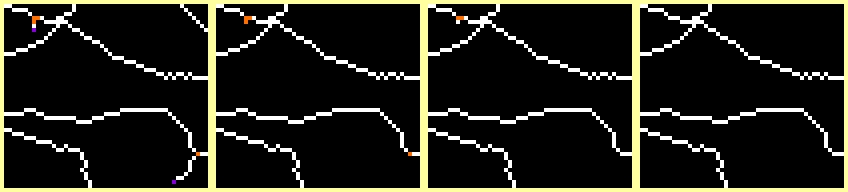
\includegraphics[width=1\textwidth]{fig/PruningStack--Montage.jpg}
\end{figure}
\item[Circular pruning]\hfill\\
Sometimes, especially when the cross-section of the tubes is large the skeletonization can lead to (small) false circular skeleton parts. If this is the case in your data try the "Prune cycle method" options of \ijmenu{Plugins > Skeleton > Analyze Skeleton (2D/3D)} and check if it  helped removing the false cycles.\\

\underline{Note}: One may consider additional algorithms; for instance to only remove branches up to a specified minimum length, however this is currently not implemented in \ijmenu{Analyze Skeleton (2D/3D)}. You should be very cautious with the pruning as important features of the network such as real loops and end point segments may also be removed. Using it or not boils down to a trade-off between removing spurious branches and removing real network branches. It is always better to try to obtain a good segmentation mask in the first place but, as you will notice, it is not easy to properly segment small and large vessels with such a simple image processing pipeline.

\item[Fill Holes]\hfill\\
The cycles in the large vessels usually originate from holes inside the segmented vessels, the problem can hence be mitigated by filling these holes in the binary mask before the skeletonization. This can be performed either in the 3D domain with \ijmenu{Plugins > 3D > 3D Fill Holes} or in 2D with \ijmenu{Process > Binary > Fill Holes}. In this last case we must specify in the command call that the operation should be applied to the whole stack (slice by slice). 

\underline{Note}:
More pixels will always be filled when the operation is performed in 2D, as a 2D hole appearing in a particular slice (e.g. a disk inside a cylinder) is not necessarily part of a 3D hole (the converse being true). In turn, 2D hole filling can generate some artifacts if the vessels form closed loops. 

\item[Morphological Closing] Sometimes the large vessels of the binary mask are not only hollow but a hole is pierced in their outside. These defects can lead to spurious small branches in the skeleton (as we saw before). If the holes are not too large they can be filled in by morphological closing of the binary mask. If you have time you can try this out.
\end{description}

\textbf{\underline{Note}} : The simple workflow proposed in this practical is working reasonably well on the datasets we acquired, but, as we saw, it is pretty limited when it comes to segment a mixture of thin and thick vessels in the same stack. It cannot compete with some high accuracy filament tracing methods, some of which are reviewed in \cite{lesage2009review}. More specifically, a very clever method is described in \cite{li2006vessels}.